\documentclass[a4paper]{article}

\def\npart {IA}
\def\nterm {Lent}
\def\nyear {2015}
\def\nlecturer {W.\ T.\ Gowers}
\def\ncourse {Analysis I}

\input{header}

\begin{document}
\maketitle
\section{The Riemann Integral}
Finally, we can get to integrals. There are many ways to define an integral, which can have some subtle differences. The definition we will use here is the \emph{Riemann integral}, which is the simplest definition, but is also the weakest one, in the sense that many functions are \emph{not} Riemann integrable but integrable under other definitions.

Still, the definition of the Riemann integral is not too straightforward, and requires a lot of preliminary definitions.
\subsection{Riemann Integral}
\begin{defi}[Dissections]
  Let $[a, b]$ be a closed interval. A \emph{dissection} of $[a, b]$ is a sequence $a = x_0 < x_1 < x_2 < \cdots < x_n = b$.
\end{defi}

\begin{defi}[Upper and lower sums]
  Given a dissection $\mathcal{D}$, the \emph{upper sum} and \emph{lower sum} are defined by the formulae
  \begin{align*}
    U_\mathcal{D} (f) &= \sum_{i = 1}^{n}(x_i - x_{i - 1}) \sup_{x\in [x_{i - 1}, x_{i}]}f (x)\\
    L_\mathcal{D} (f) &= \sum_{i = 1}^{n}(x_i - x_{i - 1}) \inf_{x\in [x_{i - 1}, x_{i}]}f (x)
  \end{align*}
  Sometimes we use the shorthand
  \[
    M_i = \sup_{x\in [x_{i - 1}, x_i]} f(x), \quad m_i = \inf_{x\in [x_{i - 1} - x_i]} f(x).
  \]
\end{defi}
The upper sum is the total area of the red rectangles, while the lower sum is the total area of the black rectangles:
\begin{center}
  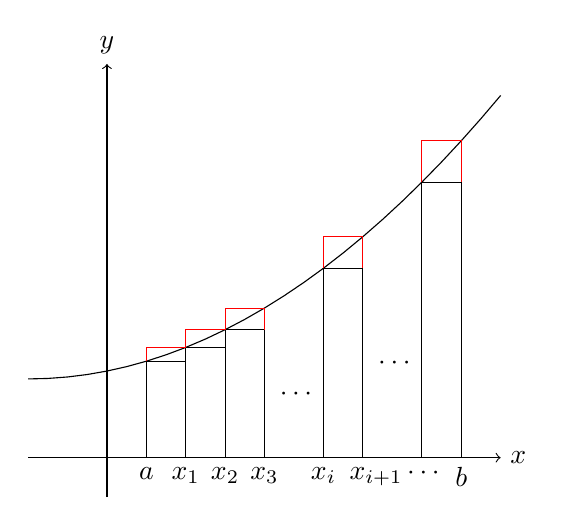
\begin{tikzpicture}
    \draw [->] (-1, 0) -- (5, 0) node [right] {$x$};
    \draw [->] (0, -0.5) -- (0, 5) node [above] {$y$};

    \draw [domain=-1:5] plot (\x, {(\x + 1)*(\x + 1)/10 + 1});

    \draw (0.5, 0) node [below] {$a$} -- (0.5, 1.225) -- (1, 1.225);
    \draw (1, 0) node [below] {$x_1$} -- (1, 1.4) -- (1.5, 1.4);
    \draw (1.5, 0) node [below] {$x_2$} -- (1.5, 1.625) -- (2, 1.625) -- (2, 0) node [below] {$x_3$};
    \node at (2.4, 0.8) {$\cdots$};
    \draw (2.75, 0) node [below] {$x_i$} -- (2.75, 2.40625) -- (3.25, 2.40625) -- (3.25, 0) node [anchor = north west] {$\!\!\!\!\!x_{i + 1}\cdots$};
    \node at (3.65, 1.2) {$\cdots$};
    \draw (4, 0) -- (4, 3.5) -- (4.5, 3.5) -- (4.5, 0) node [below] {$b$};

    \draw [red] (0.5, 1.225) -- (0.5, 1.4) -- (1, 1.4) -- (1, 1.625) -- (1.5, 1.625) -- (1.5, 1.9) -- (2, 1.9) -- (2, 1.625);
    \draw [red] (2.75, 2.40625) -- (2.75, 2.80625) -- (3.25, 2.80625) -- (3.25, 2.40625);
    \draw [red] (4, 3.5) -- (4, 4.025) -- (4.5, 4.025) -- (4.5, 3.5);
  \end{tikzpicture}
\end{center}

\begin{defi}[Refining dissections]
  If $\mathcal{D}_1$ and $\mathcal{D}_2$ are dissections of $[a, b]$, we say that $\mathcal{D}_2$ refines $\mathcal{D}_1$ if every point of $\mathcal{D}_1$ is a point of $\mathcal{D}_2$.
\end{defi}

\begin{lemma}[Refinement improves bounds]
  If $\mathcal{D}_2$ refines $\mathcal{D}_1$, then
  \[
    U_{\mathcal{D}_2} f \leq U_{\mathcal{D}_1}f\text{ and }L_{\mathcal{D}_2 f}\geq L_{\mathcal{D}_1}f.
  \]
\end{lemma}
Using the picture above, this is because if we cut up the dissections into smaller pieces, the red rectangles can only get chopped into shorter pieces and the black rectangles can only get chopped into taller pieces.
\begin{center}
  \begin{tikzpicture}
    \draw [->] (-0.5, 0) -- (3, 0) node [right] {$x$};
    \draw [->] (0, -0.5) -- (0, 3) node [above] {$y$};

    \draw [domain=-0.5:3] plot (\x, {(\x + 1)*(\x + 1)/10 + 1});

    \draw (0.5, 0) node [below] {$x_0$} -- (0.5, 1.225) -- (2, 1.225) -- (2, 0) node [below] {$x_1$};

    \draw [red] (0.5, 1.225) -- (0.5, 1.9) -- (2, 1.9) -- (2, 1.225);
    \draw [->] (3.5, 1.5) -- (4.5, 1.5);
    \begin{scope}[shift={(5.5, 0)}]
      \draw [->] (-0.5, 0) -- (3, 0) node [right] {$x$};
      \draw [->] (0, -0.5) -- (0, 3) node [above] {$y$};

      \draw [domain=-0.5:3] plot (\x, {(\x + 1)*(\x + 1)/10 + 1});

      \draw (0.5, 0) node [below] {$x_0$} -- (0.5, 1.225) -- (1, 1.225);
      \draw (1, 0) node [below] {$x_1$} -- (1, 1.4) -- (1.5, 1.4);
      \draw (1.5, 0) node [below] {$x_2$} -- (1.5, 1.625) -- (2, 1.625) -- (2, 0) node [below] {$x_3$};

      \draw [red] (0.5, 1.225) -- (0.5, 1.4) -- (1, 1.4) -- (1, 1.625) -- (1.5, 1.625) -- (1.5, 1.9) -- (2, 1.9) -- (2, 1.625);

    \end{scope}
  \end{tikzpicture}
\end{center}

\begin{proof}
  Let $\mathcal{D}$ be $x_0 < x_1 < \cdots < x_n$. Let $\mathcal{D}_2$ be obtained from $\mathcal{D}_1$ by the addition of one point $z$. If $z\in (x_{i - 1}, x_i)$, then
  \begin{align*}
    U_{\mathcal{D}_2}f - U_{\mathcal{D}_1}f &= \left[(z - x_{i - 1}) \sup_{x\in [x_{i - 1}, z]} f(x)\right]\\
    &+ \left[(x_i - z)\sup_ {x\in[z, x_i]}f(x)\right] - (x_i - x_{i - 1})M_i.
  \end{align*}
  But $\sup_{x\in [x_{i - 1}, z]} f(x)$ and $\sup_{x\in [z, x_i]} f(x)$ are both at most $M_i$. So this is at most $M_i( z - x_{i - 1} + x_i - z - (x_i - x_{i - 1})) =0 $. So
  \[
    U_{\mathcal{D}_2} f\leq U_{\mathcal{D}_1}f.
  \]
  By induction, the result is true whenever $\mathcal{D}_2$ refines $\mathcal{D}_1$.

  A very similar argument shows that $L_{\mathcal{D}_2f} \geq L_{\mathcal{D}_1}f$.
\end{proof}
\begin{defi}[Least common refinement]
  If $\mathcal{D}_1$ and $\mathcal{D}_2$ be dissections of $[a, b]$. Then the least common refinement of $\mathcal{D}_1$ and $\mathcal{D}_2$ is the dissection made out of the points of $\mathcal{D}_1$ and $\mathcal{D}_2$.
\end{defi}

\begin{cor}
  Let $\mathcal{D}_1$ and $\mathcal{D}_2$ be two dissections of $[a, b]$. Then
  \[
    U_{\mathcal{D}_1}f \geq L_{\mathcal{D}_2}f.
  \]
\end{cor}
\begin{proof}
  Let $\mathcal{D}$ be the least common refinement (or indeed any common refinement). Then by lemma above (and by definition),
  \[
    U_{\mathcal{D}_1}f \geq U_{\mathcal{D}}f \geq L_{\mathcal{D}}f \geq L_{\mathcal{D}_2}f.\qedhere
  \]
\end{proof}

Finally, we can define the integral.
\begin{defi}[Upper, lower, and Riemann integral]
  The \emph{upper integral} is
  \[
    \overline{\int_a^b} f(x)\;\d x = \inf_{\mathcal{D}}U_{\mathcal{D}}f.
  \]
  The \emph{lower integral} is
  \[
    \underline{\int_a^b} f(x)\;\d x = \sup_{\mathcal{D}}L_{\mathcal{D}}f.
  \]
  If these are equal, then we call their common value the \emph{Riemann integral} of $f$, and is denoted $\int_a^b f(x)\;\d x$.

  If this exists, we say $f$ is \emph{Riemann integrable}.
\end{defi}
We will later prove the \emph{fundamental theorem of calculus}, which says that integration is the reverse of differentiation. But why don't we simply define integration as anti-differentiation, and prove that it is the area of the curve? There are things that we cannot find (a closed form of) the anti-derivative of, like $e^{-x^2}$. In these cases, we wouldn't want to say the integral doesn't exist --- it surely does according to this definition!

There is an immediate necessary condition for Riemann integrability --- boundedness. If $f$ is unbounded above in $[a, b]$, then for any dissection $\mathcal{D}$, there must be some $i$ such that $f$ is unbounded on $[x_{i - 1}, x_i]$. So $M_i = \infty$. So $U_\mathcal{D} f = \infty$. Similarly, if $f$ is unbounded below, then $L_{\mathcal{D}} f = -\infty$. So unbounded functions are not Riemann integrable.

\begin{eg}[Integral of $x$ via definition]
  Let $f(x) = x$ on $[a, b]$. Intuitively, we know that the integral is $(b^2 - a^2)/2$, and we will show this using the definition above. Let $\mathcal{D} = x_0 < x_1 < \cdots < x_n$ be a dissection. Then
  \begin{align*}
    U_{\mathcal{D}}f &= \sum_{i = 1}^n (x_i - x_{i - 1})x_i\\
    \intertext{We \emph{know} that the integral is $\frac{b^2 - a^2}{2}$. So we put each term of the sum into the form $\frac{x_i^2 - x_{i - 1}^2}{2}$ plus some error terms.}
    &= \sum_{i = 1}^n \left(\frac{x_i^2}{2} - \frac{x_{i - 1}^2}{2} + \frac{x_i^2}{2} - x_{i - 1}x_i + \frac{x_{i - 1}^2}{2}\right)\\
    &= \frac{1}{2}\sum_{i = 1}^n (x_i^2 - x_{i - 1}^2 + (x_i - x_{i - 1})^2)\\
    &= \frac{1}{2}(b^2 - a^2) + \frac{1}{2}\sum_{i = 1}^n(x_i - x_{i - 1})^2.
  \end{align*}
  \begin{defi}[Mesh]
    The \emph{mesh} of a dissection $\mathcal{D}$ is $\max_i (x_{i+1} - x_i)$.
  \end{defi}
  Then if the mesh is $ < \delta$, then
    \[
      \frac{1}{2}\sum_{i = 1}^n (x_i - x_{i - 1})^2 \leq \frac{\delta}{2}\sum_{i = 1}^n (x_i - x_{i - 1}) = \frac{\delta}{2}(b - a).
    \]
  So by making $\delta$ small enough, we can show that for any $\varepsilon > 0$,
  \[
    \overline{\int_a^b} x\;\d x < \frac{1}{2}(b^2 - a^2) + \varepsilon.
  \]
  Similarly,
  \[
    \underline{\int_a^b} x\;\d x > \frac{1}{2}(b^2 - a^2) - \varepsilon.
  \]
  So
  \[
    \int_a^b x\;\d x = \frac{1}{2}(b^2 - a^2).
  \]
\end{eg}

\begin{eg}[Dirichlet function not integrable]
  Define $f: [0, 1] \to \R$ by
  \[
    f(x) =
    \begin{cases}
      1 & x \in \Q\\
      0 & x \not\in \Q
    \end{cases}.
  \]
  Let $x_0 < x_1 < \cdots < x_n$ be a dissection. Then for every $i$, we have $m_i = 0$ (since there is an irrational in every interval), and $M_i = 1$ (since there is a rational in every interval). So
  \[
    U_{\mathcal{D}}f = \sum_{i = 1}^nM_i(x_i - x_{i - 1}) = \sum_{i = 1}^n (x_i - x_{i - 1}) = 1.
  \]
  Similarly, $L_\mathcal{D} f = 0$. Since $\mathcal{D}$ was arbitrary, we have
  \[
    \overline{\int_0^1}f(x)\;\d x = 1, \quad \underline{\int_0^1}f(x)\;\d x = 0.
  \]
  So $f$ is \emph{not} Riemann integrable.

  Of course, this function is not interesting at all. The whole point of its existence is to show undergraduates that there are some functions that are not integrable!
\end{eg}

Note that it is important to say that the function is not \emph{Riemann} integrable. There are other notions for integration in which this function is integrable. For example, this function is \emph{Lebesgue-integrable}.

Using the definition to show integrability is often cumbersome. Most of the time, we use the \emph{Riemann's integrability criterion}, which follows rather immediately from the definition, but is much nicer to work with.
\begin{prop}[Riemann's integrability criterion]
  This is sometimes known as Cauchy's integrability criterion.

  Let $f: [a, b] \to \R$. Then $f$ is Riemann integrable if and only if for every $\varepsilon > 0$, there exists a dissection $\mathcal{D}$ such that
  \[
    U_\mathcal{D} - L_\mathcal{D} < \varepsilon.
  \]
\end{prop}

\begin{proof}
  $(\Rightarrow)$ Suppose that $f$ is integrable. Then (by definition of Riemann integrability), there exist $\mathcal{D}_1$ and $\mathcal{D}_2$ such that
  \[
    U_{\mathcal{D}_1} < \int_a^b f(x)\;\d x + \frac{\varepsilon}{2},
  \]
  and
  \[
    L_{\mathcal{D}_2} > \int_a^b f(x)\;\d x - \frac{\varepsilon}{2}.
  \]
  Let $\mathcal{D}$ be a common refinement of $\mathcal{D}_1$ and $\mathcal{D}_2$. Then
  \[
    U_\mathcal{D} f - L_\mathcal{D} f \leq U_{\mathcal{D}_1} f- L_{\mathcal{D}_2} f < \varepsilon.
  \]
  $(\Leftarrow)$ Conversely, if there exists $\mathcal{D}$ such that
  \[
    U_\mathcal{D} f - L_\mathcal{D}f < \varepsilon,
  \]
  then
  \[
    \inf U_\mathcal{D} f - \sup L_\mathcal{D} f < \varepsilon,
  \]
  which is, by definition, that
  \[
    \overline{\int_a^b} f(x)\;\d x - \underline{\int_a^b} f(x)\;\d x < \varepsilon.
  \]
  Since $\varepsilon > 0$ is arbitrary, this gives us that
  \[
    \overline{\int_a^b} f(x)\;\d x = \underline{\int_a^b} f(x)\;\d x.
  \]
  So $f$ is integrable.
\end{proof}

The next big result we want to prove is that integration is linear, ie
\[
  \int_a^b (\lambda f(x) + \mu g(x))\;\d x = \lambda\int_a^b f(x)\;\d x + \mu\int_a^bg(x)\;\d x.
\]
We do this step by step:
\begin{prop}[Scalar multiplication of integrals]
  Let $f: [a, b] \to \R$ be integrable, and $\lambda \geq 0$. Then $\lambda f$ is integrable, and
  \[
    \int_a^b \lambda f(x)\;\d x = \lambda\int_a^b f(x)\;\d x.
  \]
\end{prop}

\begin{proof}
  Let $\mathcal{D}$ be a dissection of $[a, b]$. Since
  \[
    \sup_{x\in [x_{i - 1}, x_i]}\lambda f(x) = \lambda\sup_{x\in [x_{i - 1}, x_i]}f(x),
  \]
  and similarly for inf, we have
  \begin{align*}
    U_{\mathcal{D}}(\lambda f) &= \lambda U_{\mathcal{D}} f\\
    L_{\mathcal{D}}(\lambda f) &= \lambda L_\mathcal{D} f.
  \end{align*}
  So if we choose $\mathcal{D}$ such that $U_{\mathcal{D}}f - L_\mathcal{D} f < \varepsilon/\lambda$, then $U_\mathcal{D}(\lambda f) - L_\mathcal{D}(\lambda f) < \varepsilon$. So the result follows from Riemann's integrability criterion.
\end{proof}

\begin{prop}[Negation of integrals]
  Let $f: [a, b] \to \R$ be integrable. Then $-f$ is integrable, and
  \[
    \int_a^b -f(x)\;\d x = -\int_a^bf(x)\;\d x.
  \]
\end{prop}

\begin{proof}
  Let $\mathcal{D}$ be a dissection. Then
  \begin{align*}
    \sup_{x\in [x_{i - 1}, x_i]}-f(x) &= -\inf_{x\in [x_{i - 1}, x_i]} f(x)\\
    \inf_{x\in [x_{i - 1}, x_i]}-f(x) &= -\sup_{x\in [x_{i - 1}, x_i]} f(x).
  \end{align*}
  Therefore
  \[
    U_\mathcal{D}(-f) = \sum_{i = 1}^n (x_i - x_{i - 1})(-m_i) = -L_\mathcal{D}(f).
  \]
  Similarly,
  \[
    L_\mathcal{D}(-f) = -U_\mathcal{D}f.
  \]
  So
  \[
    U_\mathcal{D}(-f) - L_\mathcal{D}(-f) = U_\mathcal{D}f - L_\mathcal{D}f.
  \]
  Hence if $f$ is integrable, then $-f$ is integrable by the Riemann integrability criterion.
\end{proof}

\begin{prop}[Linearity of integrals]
  Let $f, g: [a, b] \to \R$ be integrable. Then $f + g$ is integrable, and
  \[
    \int_a^b(f(x) + g(x))\;\d x = \int_a^b f(x)\;\d x + \int_a^b g(x)\;\d x.
  \]
\end{prop}

\begin{proof}
  Let $\mathcal{D}$ be a dissection. Then
  \begin{align*}
    U_\mathcal{D}(f + g) &= \sum_{i = 1}^n (x_i - x_{i - 1})\sup_{x\in [x_{i - 1}, x_i]}(f(x) + g(x))\\
    &\leq \sum_{i = 1}^n (x_i - x_{i - 1}) \left(\sup_{u\in [x_{i - 1}, x_i]}f(u) + \sup_{v\in [x_{i - 1}, x_i]}g(v)\right)\\
    &= U_\mathcal{D}f + U_\mathcal{D} g
  \end{align*}
  Therefore,
  \[
    \overline{\int_a^b}(f(x) + g(x))\;\d x \leq \overline{\int_a^b} f(x)\;\d x + \overline{\int_a^b} g(x)\;\d x = \int_a^b f(x)\;\d x + \int_a^bg(x)\;\d x.
  \]
  Similarly,
  \[
  \underline{\int_a^b}(f(x) + g(x))\;\d x \geq \int_a^b f(x)\;\d x + \int_a^b g(x)\;\d x.
  \]
  So the upper and lower integrals are equal, and the result follows.
\end{proof}
So we now have that
\[
  \int_a^b (\lambda f(x) + \mu g(x))\;\d x = \lambda\int_a^b f(x)\;\d x + \mu\int_a^bg(x)\;\d x.
\]
We will prove more ``obvious'' results.
\begin{prop}[Monotonicity of integrals]
  Let $f, g: [a, b] \to \R$ be integrable, and suppose that $f(x) \leq g(x)$ for every $x$. Then
  \[
    \int_a^b f(x)\;\d x \leq \int_a^b g(x)\;\d x.
  \]
\end{prop}

\begin{proof}
  Follows immediately from the definition.
\end{proof}

\begin{prop}[Absolute value preserves integrability]
  Let $f: [a, b] \to \R$ be integrable. Then $|f|$ is integrable.
\end{prop}

\begin{proof}
  Note that we can write
  \[
    \sup_{x\in [x_{i - 1}, x_i]}f(x) - \inf_{x\in [x_{i - 1}, x_i]}f(x) = \sup_{u, v\in [x_{i - 1}, x_i]}|f(u) - f(v)|.
  \]
  Similarly,
  \[
    \sup_{x\in [x_{i - 1}, x_i]}|f(x)| - \inf_{x\in [x_{i - 1}, x_i]}|f(x)| = \sup_{u, v\in [x_{i - 1}, x_i]}||f(u)| - |f(v)||.
  \]
  For any pair of real numbers, $x, y$, we have that $||x| - |y|| \leq |x - y|$ by the triangle inequality. Then for any interval $u, v\in [x_{i - 1}, x_i]$, we have
  \[
    ||f(u)| - |f(v)|| \leq |f(u) - f(v)|.
  \]
  Hence we have
  \[
    \sup_{x\in [x_{i - 1}, x_i]}|f(x)| - \inf_{x\in [x_{i - 1}, x_i]}|f(x)| \leq \sup_{x\in [x_{i - 1}, x_i]}f(x) - \inf_{x\in [x_{i - 1}, x_i]} f(x).
  \]
  So for any dissection $\mathcal{D}$, we have
  \[
    U_\mathcal{D} (|f|) - L_\mathcal{D}(|f|) \leq U_\mathcal{D}(f) - L_\mathcal{D}(f).
  \]
  So the result follows from Riemann's integrability criterion.
\end{proof}
Combining these two propositions, we get that if
\[
  |f(x) - g(x)| \leq C,
\]
for every $x\in[a, b]$, then
\[
  \left|\int_a^bf(x)\;\d x - \int_a^b g(x)\;\d x\right| \leq C(b - a).
\]

\begin{prop}[Additivity property]
  Let $f: [a, c] \to \R$ be integrable, and let $b\in (a, c)$. Then the restrictions of $f$ to $[a, b]$ and $[b, c]$ are Riemann integrable, and
  \[
    \int_a^b f(x)\;\d x + \int_b^c f(x)\;\d x = \int_a^c f(x) \;\d x
  \]
  Similarly, if $f$ is integrable on $[a, b]$ and $[b, c]$, then it is integrable on $[a, c]$ and the above equation also holds.
\end{prop}

\begin{proof}
  Let $\varepsilon> 0$, and let $a = x_0 < x_1 < \cdots < x_n = c$ be a dissection of $\mathcal{D}$ of $[a, c]$ such that
  \[
    U_\mathcal{D}(f) \leq \int_a^c f(x)\;\d x + \varepsilon,
  \]
  and
  \[
    L_\mathcal{D}(f) \geq \int_a^c f(x)\;\d x - \varepsilon.
  \]
  Let $\mathcal{D}'$ be the dissection made of $\mathcal{D}$ plus the point $b$. Let $\mathcal{D}_1$ be the dissection of $[a, b]$ made of points of $\mathcal{D}'$ from $a$ to $b$, and $D_2$ be the dissection of $[b, c]$ made of points of $\mathcal{D}'$ from $b$ to $c$. Then
  \[
    U_{\mathcal{D}_1}(f) + U_{\mathcal{D}_2}(f) = U_{\mathcal{D}'}(f) \leq U_{\mathcal{D}}(f),
  \]
  and
  \[
    L_{\mathcal{D}_1}(f) + L_{\mathcal{D}_2}(f) = L_{\mathcal{D}'}(f) \geq L_\mathcal{D} (f).
  \]
  Since $U_\mathcal{D}(f) - L_\mathcal{D}(f) < 2\varepsilon$, and both $U_{\mathcal{D}_2}(f) - L_{\mathcal{D}_2} (f)$ and $U_{\mathcal{D}_1}(f) - L_{\mathcal{D}_1} (f)$ are non-negative, we have $U_{\mathcal{D}_1} (f) - L_{\mathcal{D}_1} (f)$ and $U_{\mathcal{D}_2}(f) - L_{\mathcal{D}_2}(f)$ are less than $2\varepsilon$. Since $\varepsilon$ is arbitrary, it follows that the restrictions of $f$ to $[a, b]$ and $[b, c]$ are both Riemann integrable. Furthermore,
  \begin{multline*}
    \int_a^b f(x)\;\d x + \int_b^c f(x)\;\d x \leq U_{\mathcal{D}_1}(f) + U_{\mathcal{D}_2}(f) = U_{\mathcal{D}'}(f) \leq U_{\mathcal{D}}(f)\\
    \leq \int_a^c f(x)\;\d x + \varepsilon.
  \end{multline*}
  Similarly,
  \begin{multline*}
    \int_a^bf(x)\;\d x + \int_b^cf(x)\;\d x \geq L_{\mathcal{D}_1}(f) + L_{\mathcal{D}_2}(f) = L_{\mathcal{D}'}(f) \geq L_{\mathcal{D}}(f)\\
    \geq \int_a^c f(x)\;\d x - \varepsilon.
  \end{multline*}
  Since $\varepsilon$ is arbitrary, it follows that
  \[
    \int_a^b f(x)\;\d x + \int_b^c f(x)\;\d x = \int_a^c f(x)\;\d x.
  \]
  The other direction is left as an (easy) exercise.
\end{proof}

\begin{prop}[Product of integrable functions]
  Let $f, g: [a, b] \to \R$ be integrable. Then $fg$ is integrable.
\end{prop}

\begin{proof}
  Let $C$ be such that $|f(x)|, |g(x)| \leq C$ for every $x\in [a, b]$. Write $L_i$ and $\ell_i$ for the $\sup$ and $\inf$ of $g$ in $[x_{i - 1}, x_i]$. Now let $\mathcal{D}$ be a dissection, and for each $i$, let $u_i$ and $v_i$ be two points in $[x_{i - 1}, x_i]$.

  We will pretend that $u_i$ and $v_i$ are the minimum and maximum when we write the proof, but we cannot assert that they are, since $fg$ need not have maxima and minima. We will then note that since our results hold for arbitrary $u_i$ and $v_i$, it must hold when $fg$ is at its supremum and infimum.

  We find what we pretend is the difference between the upper and lower sum:
  \begin{align*}
    &\quad \left|\sum_{i = 1}^n \big(x_i - x_{i - 1})(f(v_i)g(v_i) - f(u_i)g(u_i)\big)\right| \\
    &= \left|\sum_{i = 1}^{n}(x_i - x_{i - 1})\big(f(v_i)(g(v_i) - g(u_i)) + (f(v_i) - f(u_i))g(u_i)\big)\right|\\
    &\leq \sum_{i = 1}^n \big(C(L_i - \ell_i) + (M_i - m_i)C\big)\\
    &=C(U_\mathcal{D}g - L_\mathcal{D}g + U_\mathcal{D}f - L_\mathcal{D}f).
  \end{align*}
  Since $u_i$ and $v_i$ are arbitrary, it follows that
  \[
    U_\mathcal{D}(fg) - L_\mathcal{D}(fg) \leq C(U_\mathcal{D}f - L_\mathcal{D}f + U_\mathcal{D}g - L_\mathcal{D}g).
  \]
  Since $C$ is fixed, and we can get $U_\mathcal{D} f - L_\mathcal{D}f$ and $U_\mathcal{D}g - L_\mathcal{D}g$ arbitrary small (since $f$ and $g$ are integrable), we can get $U_\mathcal{D}(fg) - L_\mathcal{D}(fg)$ arbitrarily small. So the result follows.
\end{proof}

\begin{thm}[Continuous functions are integrable]
  Every continuous function $f$ on a closed bounded interval $[a, b]$ is Riemann integrable.
\end{thm}

\begin{proof}
  wlog assume $[a, b] = [0, 1]$.

  Suppose the contrary. Let $f$ be non-integrable. This means that there exists some $\varepsilon$ such that for every dissection $\mathcal{D}$, $U_{\mathcal{D}} - L_{\mathcal{D}} > \varepsilon$. In particular, for every $n$, let $\mathcal{D}_n$ be the dissection $0, \frac{1}{n}, \frac{2}{n}, \cdots, \frac{n}{n}$.

  Since $U_{\mathcal{D}_n} - L_{\mathcal{D}_n} > \varepsilon$, there exists some interval $\left[\frac{k}{n}, \frac{k + 1}{n}\right]$ in which $\sup f - \inf f > \varepsilon$. Suppose the supremum and infimum are attained at $x_n$ and $y_n$ respectively. Then we have $|x_n - y_n| < \frac{1}{n}$ and $f(x_n) - f(y_n) > \varepsilon$.

  By Bolzano Weierstrass, $(x_n)$ has a convergent subsequence, say $(x_{n_i})$. Say $x_{n_i}\to x$. Since $|x_n - y_n| < \frac{1}{n}\to 0$, we must have $y_{n_i}\to x$. By continuity, we must have $f(x_{n_i}) \to f(x)$ and $f(y_{n_i}) \to f(x)$, but $f(x_{n_i})$ and $f(y_{n_i})$ are always apart by $\varepsilon$. Contradiction.
\end{proof}
With this result, we know that a lot of things are integrable, e.g.\ $e^{-x^2}$.

To prove this, we secretly used the property of \emph{uniform continuity}:
\begin{defi}[Uniform continuity*]
  Let $A\subseteq \R$ and let $f: A\to \R$. Then $f$ is \emph{uniformly continuous} if
  \[
    (\forall \varepsilon)(\exists \delta > 0)(\forall x)(\forall y)\;|x - y| < \delta \Rightarrow |f(x) - f(y)| \leq \varepsilon.
  \]
\end{defi}
This is different from regular continuity. Regular continuity says that at any point $x$, we can find a $\delta$ that works for this point. Uniform continuity says that we can find a $\delta$ that works for \emph{any} $x$.

It is easy to show that a uniformly continuous function is integrable, since by uniformly continuity, as long as the mesh of a dissection is sufficiently small, the difference between the upper sum and the lower sum can be arbitrarily small by uniform continuity. Thus to prove the above theorem, we just have to show that continuous functions on a closed bounded interval are uniformly continuous.

\begin{thm}[non-examinable]
  Let $a < b$ and let $f: [a, b] \to \R$ be continuous. Then $f$ is uniformly continuous.
\end{thm}

\begin{proof}
  Suppose that $f$ is not uniformly continuous. Then
  \[
    (\exists \varepsilon)(\forall \delta > 0)(\exists x)(\exists y)\;|x - y| < \delta \text{ and } |f(x) - f(y)| \geq \varepsilon.
  \]
  Therefore, we can find sequences $(x_n), (y_n)$ such that for every $n$, we have
  \[
    |x_n - y_n| \leq \frac{1}{n}\text{ and }|f(x_n) - f(y_n)| \geq \varepsilon.
  \]
  Then by Bolzano-Weierstrass theorem, we can find a subsequence $(x_{n_k})$ converging to some $x$. Since $|x_{n_k} - y_{n_k}| \leq \frac{1}{n_k}$, $y_{n_k}\to x$ as well. But $|f(x_{n_k}) - f(y_{n_k})| \geq \varepsilon$ for every $k$. So $f(x_{n_k})$ and $f(y_{n_k})$ cannot both converge to the same limit. So $f$ is not continuous at $x$.
\end{proof}
This proof is very similar to the proof that continuous functions are integrable. In fact, the proof that continuous functions are integrable is just a fuse of this proof and the (simple) proof that uniformly continuously functions are integrable.

\begin{thm}[Monotone functions are integrable]
  Let $f: [a, b] \to \R$ be monotone. Then $f$ is Riemann integrable.
\end{thm}
Note that monotone functions need not be ``nice''. It can even have infinitely many discontinuities. For example, if $f: [0, 1] \to \R$ maps $x$ to the $1/(\text{first non-zero digit in the binary expansion of }x)$, with $f(0) = 0$.

\begin{proof}
  let $\varepsilon > 0$. Let $\mathcal{D}$ be a dissection of mesh less than $\frac{\varepsilon}{f(b) - f(a)}$. Then
  \begin{align*}
    U_\mathcal{D} f - L_\mathcal{D}f &= \sum_{i = 1}^n (x_i - x_{i - 1})(f(x_i) - f(x_{i - 1}))\\
    &\leq \frac{\varepsilon}{f(b) - f(a)} \sum_{i = 1}^n (f(x_i) - f(x_{i - 1}))\\
    &= \varepsilon.\qedhere
  \end{align*}
\end{proof}

Pictorially, we see that the difference between the upper and lower sums is total the area of the red rectangles.
\begin{center}
  \begin{tikzpicture}
    \draw [->] (-1, 0) -- (5, 0) node [right] {$x$};
    \draw [->] (0, -0.5) -- (0, 5) node [above] {$y$};

    \draw [domain=-1:5] plot (\x, {(\x + 1)*(\x + 1)/10 + 1});

    \draw (0.5, 0) rectangle (1, 1.225);
    \draw (1, 0) rectangle (1.5, 1.4);
    \draw (1.5, 0) rectangle (2, 1.625);
    \draw (2, 0) rectangle (2.5, 1.9);
    \draw (2.5, 0) rectangle (3, 2.225);
    \draw (3, 0) rectangle (3.5, 2.6);
    \draw (3.5, 0) rectangle (4, 3.026);
    \draw (4, 0) rectangle (4.5, 3.5);

    \draw [red] (0.5, 1.225) rectangle (1, 1.4);
    \draw [red] (1, 1.4) rectangle (1.5, 1.625);
    \draw [red] (1.5, 1.625) rectangle (2, 1.9);
    \draw [red] (2, 1.9) rectangle (2.5, 2.225);
    \draw [red] (2.5, 2.225) rectangle (3, 2.6);
    \draw [red] (3, 2.6) rectangle (3.5, 3.025);
    \draw [red] (3.5, 3.025) rectangle (4, 3.5);
    \draw [red] (4, 3.5) rectangle (4.5, 4.025);
  \end{tikzpicture}
\end{center}
To calculate the total area, we can stack the red areas together to get something of width $\frac{\varepsilon}{f(b) - f(a)}$ and height $f(b) - f(a)$. So the total area is just $\varepsilon$.

\begin{lemma}[Integrability on interior]
  Let $a < b$ and let $f$ be a bounded function from $[a, b] \to \R$ that is continuous on $(a, b)$. Then $f$ is integrable.
\end{lemma}
An example where this would apply is $\int_0^1 \sin \frac{1}{x}$. It gets nasty near $x = 0$, but its ``nastiness'' is confined to $x = 0$ only. So as long as its nastiness is sufficiently contained, it would still be integrable.

The idea of the proof is to integrate from a point $x_1$ very near $a$ up to a point $x_{n - 1}$ very close to $b$. Since $f$ is bounded, the regions $[a, x_1]$ and $[x_{n - 1}, b]$ are small enough to not cause trouble.

\begin{proof}
  Let $\varepsilon > 0$. Suppose that $|f(x)| \leq C$ for every $x\in [a, b]$. Let $x_0 = a$ and pick $x_1$ such that $x_1 - x_0 < \frac{\varepsilon}{8C}$. Also choose $z$ between $x_1$ and $b$ such that $b - z < \frac{\varepsilon}{8C}$.

  Then $f$ is continuous $[x_1, z]$. Therefore it is integrable on $[x_1, z]$. So we can find a dissection $\mathcal{D}'$ with points $x_1 < x_2 < \cdots < x_{n - 1} = z$ such that
  \[
    U_{\mathcal{D}'}f - L_{\mathcal{D}'}f < \frac{\varepsilon}{2}.
  \]
  Let $\mathcal{D}$ be the dissection $a = x_0 < x_1 < \cdots < x_n = b$. Then
  \[
    U_\mathcal{D} f - L_\mathcal{D} f < \frac{\varepsilon}{8C}\cdot 2C + \frac{\varepsilon}{2} + \frac{\varepsilon}{8C}\cdot 2C = \varepsilon.
  \]
  So done by Riemann integrability criterion.
\end{proof}

\begin{eg}[Integrable functions with discontinuities]\leavevmode
  \begin{itemize}
    \item $f(x) =
      \begin{cases}
        \sin \frac{1}{x}& x \not = 0\\
        0 & x = 0
      \end{cases}$ defined on $[-1, 1]$ is integrable.
    \item $g(x) =
      \begin{cases}
        x & x \leq 1\\
        x^2 + 1 & x > 1
      \end{cases}$ defined on $[0, 1]$ is integrable.
  \end{itemize}
\end{eg}

\begin{cor}
  Every piecewise continuous and bounded function on $[a, b]$ is integrable.
\end{cor}

\begin{proof}
  Partition $[a, b]$ into intervals $I_1, \cdots, I_k$, on each of which $f$ is (bounded and) continuous. Hence for every $I_j$ with end points $x_{j - 1}$, $x_j$, $f$ is integrable on $[x_{j - 1}, x_j]$ (which may not equal $I_j$, e.g.\ $I_j$ could be $[x_{j - 1}, x_j)$). But then by the additivity property of integration, we get that $f$ is integrable on $[a, b]$
\end{proof}

We defined Riemann integration in a very general way --- we allowed \emph{arbitrary} dissections, and took the extrema over all possible dissection. Is it possible to just consider some particular nice dissections instead? Perhaps unsurprisingly, yes! It's just that we opt to define it the general way so that we can easily talk about things like least common refinements.
\begin{lemma}[Uniform dissections converge to integral]
  Let $f: [a, b] \to \R$ be Riemann integrable, and for each $n$, let $\mathcal{D}_n$ be the dissection $a = x_0 < x_1 < \cdots < x_n = b$, where $x_i = a + \frac{i(b - a)}{n}$ for each $i$. Then
  \[
    U_{\mathcal{D}_n}f \to \int_a^b f(x)\;\d x
  \]
  and
  \[
    L_{\mathcal{D}_n}f \to \int_a^b f(x)\;\d x.
  \]
\end{lemma}

\begin{proof}
  Let $\varepsilon > 0$. We need to find an $N$. The only thing we know is that $f$ is Riemann integrable, so we use it:

  Since $f$ is integrable, there is a dissection $\mathcal{D}$, say $u_0 < u_1 < \cdots < u_m$, such that
  \[
    U_\mathcal{D} f - \int_a^b f(x)\;\d x < \frac{\varepsilon}{2}.
  \]
  We also know that $f$ is bounded. Let $C$ be such that $|f(x)| \leq C$.

  For any $n$, let $\mathcal{D}'$ be the least common refinement of $\mathcal{D}_n$ and $\mathcal{D}$. Then
  \[
    U_{\mathcal{D}'}f \leq U_\mathcal{D} f.
  \]
  Also, the sums $U_{\mathcal{D}_n}f$ and $U_\mathcal{D'}f$ are the same, except that at most $m$ of the subintervals $[x_{i - 1}, x_i]$ are subdivided in $\mathcal{D}'$.

  For each interval that gets chopped up, the upper sum decreases by at most $\frac{b - a}{n}\cdot 2C$. Therefore
  \[
    U_{\mathcal{D}_n}f - U_{\mathcal{D}'}f \leq \frac{b - a}{n}2C\cdot m.
  \]
  Pick $n$ such that $2Cm(b - a)/n < \frac{\varepsilon}{2}$. Then
  \[
    U_{\mathcal{D}_n} f - U_\mathcal{D}f < \frac{\varepsilon}{2}.
  \]
  So
  \[
    U_{\mathcal{D}_n}f - \int_a^b f(x)\;\d x < \varepsilon.
  \]
  This is true whenever $n > \frac{4C(b - a)m}{\varepsilon}$. Since we also have $U_{\mathcal{D}_n} f \geq \int_a^b f(x)\;\d x$, therefore
  \[
    U_{\mathcal{D}_n}f \to \int_a^b f(x)\;\d x.
  \]
  The proof for lower sums is similar.
\end{proof}

For convenience, we define the following:
\begin{notation}
  If $b > a$, we define
  \[
    \int_b^a f(x)\;\d x = -\int_a^b f(x)\;\d x.
  \]
\end{notation}

We now prove that the fundamental theorem of calculus, which says that integration is the reverse of differentiation.
\begin{thm}[Fundamental theorem of calculus, part 1]
  Let $f: [a, b]\to \R$ be continuous, and for $x\in [a, b]$, define
  \[
    F(x) = \int_a^x f(t)\;\d t.
  \]
  Then $F$ is differentiable and $F'(x) = f(x)$ for every $x$.
\end{thm}

\begin{proof}
  \[
    \frac{F(x + h) - F(x)}{h} = \frac{1}{h}\int_x^{x + h}f(t)\;\d t
  \]
  Let $\varepsilon > 0$. Since $f$ is continuous, at $x$, then there exists $\delta$ such that $|y - x| < \delta$ implies $|f(y) - f(x)| < \varepsilon$.

  If $|h| < \delta$, then
  \begin{align*}
    \left|\frac{1}{h}\int_x^{x + h}f(t) \;\d t - f(x)\right| &= \left|\frac{1}{h}\int_x^{x + h}(f(t) - f(x))\;\d t\right|\\
    &\leq \frac{1}{|h|}\left|\int_x^{x + h}|f(t) - f(x)|\;\d t\right|\\
    &\leq \frac{\varepsilon|h|}{|h|}\\
    &= \varepsilon.\qedhere
  \end{align*}
\end{proof}

\begin{cor}
  If $f$ is continuously differentiable on $[a, b]$, then
  \[
    \int_a^b f'(t)\;\d t = f(b) - f(a).
  \]
\end{cor}

\begin{proof}
  Let
  \[
    g(x) = \int_a^x f'(t)\;\d t.
  \]
  Then
  \[
    g'(x) = f'(x) = \frac{\d }{\d x}(f(x) - f(a)).
  \]
  Since $g'(x) - f'(x) = 0$, $g(x) - f(x)$ must be a constant function by the mean value theorem. We also know that
  \[
    g(a) = 0 = f(a) - f(a)
  \]
  So we must have $g(x) = f(x) - f(a)$ for every $x$, and in particular, for $x = b$.
\end{proof}

\begin{thm}[Fundamental theorem of calculus, part 2]
  Let $f: [a, b] \to \R$ be a differentiable function, and suppose that $f'$ is integrable. Then
  \[
    \int_a^b f'(t)\;\d t = f(b) - f(a).
  \]
\end{thm}
Note that this is a stronger result than the corollary above, since it does not require that $f'$ is continuous.

\begin{proof}
  Let $\mathcal{D}$ be a dissection $x_0 < x_1 < \cdots < x_n$. We want to make use of this dissection. So write
  \[
    f(b) - f(a) = \sum_{i = 1}^n (f(x_i) - f(x_{i - 1})).
  \]
  For each $i$, there exists $u_i\in (x_{i - 1}, x_i)$ such that $f(x_i) - f(x_{i - 1j}) = (x_i - x_{i - 1})f'(u_i)$ by the mean value theorem. So
  \[
    f(b) - f(a) = \sum_{i = 1}^n (x_i - x_{i - 1})f'(u_i).
  \]
  We know that $f'(u_i)$ is somewhere between $\sup\limits_{x\in[x_i, x_{i - 1}]}f'(x)$ and $\inf\limits_{x\in[x_i, x_{i - 1}]}f'(x)$ by definition. Therefore
  \[
    L_\mathcal{D} f' \leq f(b) - f(a) \leq U_\mathcal{D} f'.
  \]
  Since $f'$ is integrable and $\mathcal{D}$ was arbitrary, $L_\mathcal{D}f'$ and $U_\mathcal{D}f'$ can both get arbitrarily close to $\int_a^b f'(t)\;\d t$. So
  \[
    f(b) - f(a) = \int_a^b f'(t)\;\d t.\qedhere
  \]
\end{proof}
Note that the condition that $f'$ is integrable is essential. It is possible to find a differentiable function whose derivative is not integrable! You will be asked to find it in the example sheet.

Using the fundamental theorem of calculus, we can easily prove integration by parts:
\begin{thm}[Integration by parts]
  Let $f, g:[a, b]\to \R$ be integrable such that everything below exists. Then
  \[
    \int_a^b f(x)g'(x)\;\d x = f(b)g(b) - f(a)g(a) - \int_a^b f'(x)g(x)\;\d x.
  \]
\end{thm}

\begin{proof}
  By the fundamental theorem of calculus,
  \[
    \int_a^b (f(x)g'(x) + f'(x)g(x))\;\d x = \int_a^b(fg)'(x)\;\d x = f(b)g(b) - f(a)g(a).
  \]
  The result follows after rearrangement.
\end{proof}

Recall that when we first had Taylor's theorem, we said it had the Lagrange form of the remainder. There are many other forms of the remainder term. Here we will look at the integral form:
\begin{thm}[Taylor's theorem with the integral form of the remainder]
  Let $f$ be $n + 1$ times differentiable on $[a, b]$ with $f^{(n + 1)}$ continuous. Then
  \begin{align*}
    f(b) &= f(a) + (b - a)f'(a) + \frac{(b - a)^2}{2!}f^{(2)}(a) + \cdots \\
    &+ \frac{(b - a)^n}{n!}f^{(n)}(a) + \int_a^b \frac{(b - t)^n}{n!}f^{(n + 1)}(t)\;\d t.
  \end{align*}
\end{thm}
\begin{proof}
  Induction on $n$.

  When $n = 0$, the theorem says
  \[
    f(b) - f(a) = \int_a^b f'(t)\;\d t.
  \]
  which is true by the fundamental theorem of calculus.

  Now observe that
  \begin{align*}
    \int_a^b \frac{(b - t)^n}{n!}f^{(n + 1)}(t)\;\d t ={}& \left[\frac{-(b - t)^{n + 1}}{(n + 1)!}f^{(n + 1)}(t)\right]_a^b\\
    &+ \int_a^b \frac{(b - t)^{n + 1}}{(n + 1)!}f^{(n + 1)}(t)\;\d t \\
    ={}& \frac{(b - a)^{n + 1}}{(n + 1)!} f^{(n + 1)}(a) + \int_a^b \frac{(b - t)^{n + 1}}{(n + 1)!}f^{(n + 2)}(t)\;\d t.
  \end{align*}
  So the result follows by induction.
\end{proof}
Note that the form of the integral remainder is rather weird and unexpected. How could we have come up with it? We might start with the fundamental theorem of algebra and integrate by parts. The first attempt would be to integrate $1$ to $t$ and differentiate $f'(t)$ to $f^{(2)}(t)$. So we have
\begin{align*}
  f(b) &= f(a) + \int_a^b f'(t)\;\d t\\
  &= f(a) + [tf'(t)]_a^b - \int_a^b tf^{(2)}(t)\;\d t\\
  &= f(a) + bf'(b) - af'(a) - \int_a^b tf^{(2)}(t)\;\d t\\
  \intertext{We want something in the form $(b - a)f'(a)$, so we take that out and see what we are left with.}
  &= f(a) + (b - a)f'(a) + b(f'(b) - f'(a)) - \int_a^b tf^{(2)}(t)\;\d t\\
  \intertext{Then we note that $f'(b) - f'(a) = \int_a^b f^{(2)}(t)\;\d t$. So we have}
  &= f(a) + (b - a)f'(a) + \int_a^b (b - t)f^{(2)}(t)\;\d t.
\end{align*}
Then we can see that the right thing to integrate is $(b - t)$ and continue to obtain the result.

\begin{thm}[Integration by substitution]
  Let $f: [a, b] \to \R$ be continuous. Let $g: [u, v] \to \R$ be continuously differentiable, and suppose that $g(u) = a, g(v) = b$, and $f$ is defined everywhere on $g([u, v])$ (and still continuous). Then
  \[
    \int_a^b f(x)\;\d x = \int_u^v f(g(t))g'(t)\;\d t.
  \]
\end{thm}

\begin{proof}
  By the fundamental theorem of calculus, $f$ has an anti-derivative $F$ defined on $g([u, v])$. Then
  \begin{align*}
    \int_u^v f(g(t))g'(t) \;\d t &= \int_u^v F'(g(t))g'(t)\;\d t \\
    &= \int_u^v (F\circ g)'(t)\;\d t \\
    &= F\circ g(v) - F\circ g(u)\\
    &= F(b) - F(a)\\
    &= \int_a^b f(x)\;\d x.\qedhere
  \end{align*}
\end{proof}
We can think of ``integration by parts'' as what you get by integrating the product rule, and ``integration by substitution'' as what you get by integrating the chain rule.

\subsection{Improper integrals}
It is sometimes sensible to talk about integrals of unbounded functions or integrating to infinity. But we have to be careful and write things down nicely.

\begin{defi}[Improper integral]
  Suppose that we have a function $f: [a, b] \to \R$ such that, for every $\varepsilon > 0$, $f$ is integrable on $[a + \varepsilon, b]$ and $\lim\limits_{\varepsilon \to 0}\int_{a + \varepsilon}^b f(x)\;\d x$ exists. Then we define the improper integral
  \[
    \int_a^bf(x)\;\d x \text{ to be } \lim_{\varepsilon \to 0}\int_{a + \varepsilon}^b f(x)\;\d x.
  \]
  even if the Riemann integral does not exist.

  We can do similarly for $[a, b - \varepsilon]$, or integral to infinity:
  \[
    \int_a^\infty f(x)\;\d x = \lim_{b \to \infty} \int_a^b f(x)\;\d x.
  \]
  when it exists.
\end{defi}
\begin{eg}[Improper integral with power singularity]
  \[
    \int_\varepsilon^1 x^{-1/2}\;\d x = \left[2x^{-1/2}\right]^1_\varepsilon = 2 - 2\varepsilon^{1/2} \to 2.
  \]
  So
  \[
    \int_0^1 x^{-1/2}\;\d x = 2,
  \]
  even though $x^{-1/2}$ is unbounded on $[0, 1]$.

  Note that officially we are required to make $f(x) = x^{-1/2}$ a function with domain $[0, 1]$. So we can assign $f(0) = \pi$, or any number, since it doesn't matter.
\end{eg}

\begin{eg}[Improper integral to infinity]
  \[
    \int_1^x \frac{1}{t^2}\;\d t = \left[-\frac{1}{t}\right]_1^x = 1 - \frac{1}{x} \to 1\text{ as }x\to \infty
  \]
  by the fundamental theorem of calculus. So
  \[
    \int_1^{\infty}\frac{1}{x^2}\;\d x = 1.
  \]
\end{eg}

Finally, we can prove the integral test, whose proof we omitted when we first began.
\begin{thm}[Integral test]
  Let $f: [1, \infty] \to \R$ be a decreasing non-negative function. Then $\sum_{n = 1}^\infty f(n)$ converges iff $\int_1^\infty f(x)\;\d x < \infty$.
\end{thm}

\begin{proof}
  We have
  \[
    \int_n^{n + 1}f(x)\;\d x \leq f(n) \leq \int_{n -1}^n f(x)\;\d x,
  \]
  since $f$ is decreasing (the right hand inequality is valid only for $n\geq 2$). It follows that
  \[
    \int_1^{N + 1}f(x)\;\d x \leq \sum_{n = 1}^N f(n) \leq \int_1^N f(x)\;\d x + f(1)
  \]
  So if the integral exists, then $\sum f(n)$ is increasing and bounded above by $\int_1^\infty f(x)\;\d x$, so converges.

  If the integral does not exist, then $\int_1^N f(x)\;\d x$ is unbounded. Then $\sum_{n = 1}^N f(n)$ is unbounded, hence does not converge.
\end{proof}

\begin{eg}[Integral test for $\sum 1/n^2$]
  Since $\int_1^x \frac{1}{t^2}\;\d t < \infty$, it follows that $\sum_{n = 1}^\infty \frac{1}{n^2}$ converges.
\end{eg}
\end{document}
